\begin{frame}{How to represent N different concepts?}
Consider the following problem of representing 
\begin{itemize} 
  \item \textcolor{red}{red triangle} 
  \item \textcolor{green}{green circle} 
  \item \textcolor{blue}{blue rectangle}
\end{itemize} \newline

Simplest possible way is to use one neuron per concept. This method is also known as \textbf{localist representation}. \newline
\end{frame}

\begin{frame}{How to represent N different concepts?}
Consider the following problem of representing 
\begin{itemize} 
  \item \textcolor{red}{red triangle} 
  \item \textcolor{green}{green circle} 
  \item \textcolor{blue}{blue rectangle}
\end{itemize} \newline

Simplest possible way is to use one neuron per concept. This method is also known as \textbf{localist representation}. \newline

What if you want to add new concepts, say, a \textcolor{blue}{blue triangle} and a \textcolor{green}{green rectangle}? Localist representation would simply add a new neuron for the concept. Can we do \textbf{better}?
\end{frame}

\begin{frame}{Distributed representation}
Key idea: let's split the representation into a \textit{\textcolor{red}{c}\textcolor{green}{o}\textcolor{blue}{l}\textcolor{red}{o}\textcolor{green}{r}} and a \textit{shape}. \newline

\begin{itemize}
	\item \textbf{Efficient}. Instead of using a neuron for each concept, use a neuron for the color and a neuron for the shape. 
	\item \textbf{Powerful}. Distributed representations can \textit{share attributes} between concepts. 
\end{itemize}
\end{frame}

\begin{frame}{Distributed representation}
Key idea: let's split the representation into a \textit{\textcolor{red}{c}\textcolor{green}{o}\textcolor{blue}{l}\textcolor{red}{o}\textcolor{green}{r}} and a \textit{shape}. \newline

\begin{itemize}
	\item \textbf{Efficient}. Instead of using a neuron for each concept, use a neuron for the color and a neuron for the shape. 
	\item \textbf{Powerful}. Distributed representations can \textit{share attributes} between concepts. 
\end{itemize} \newlinew

We've seen these before: they are exactly the hidden layers in feed-forward networks! 
\end{frame}

\begin{frame}{Distributed representation}
Some family of methods, e.g., autoencoders try to directly learn distributed representations. In addition, we can require a \textit{manifold}-structure of the representation, which allows us to perform meaningful vector algebra directly on the representation:

\centering
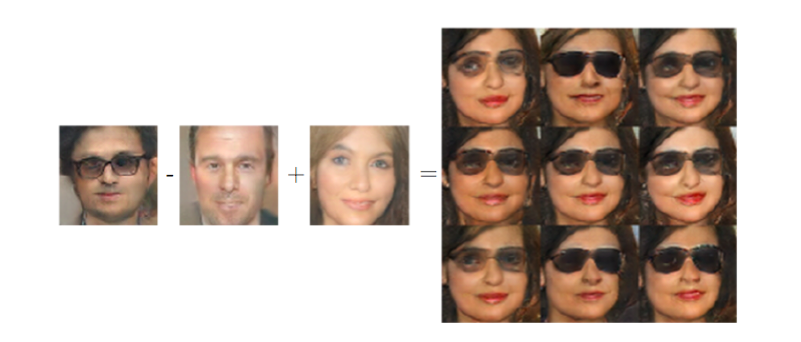
\includegraphics[width=0.9\textwidth]{figures/manifold_algebra.png}
\label{Radford et al. 2015}
\end{frame}

\begin{frame}{Distributed representation}
Why are distributed representations so powerful? \linebreak

\begin{itemize}
	\item Attribute sharing. 
	\item Distributed representation using n features with k values each can represent $k^n$ concepts. Compare this to $kn$ concepts with localist representation. 
\end{itemize}
\end{frame}

\begin{frame}{Exponential gains from depth}
How do distributed representations work combine with deep networks? \linebreak

\begin{itemize}
	\item Theoretical results say that there exist families of functions that can be efficiently represented by an architecture of depth k, but would require an exponential number of hidden units with insufficient depth. 
	\item In practice, this means that organizing computation through the composition of many nonlinearities and a hierarchy of reused features can give an exponential boost to statistical efficiency, on top of the exponential boost given by using a distributed representation.
\end{itemize}
\end{frame} 

\begin{frame}{Desirable properties of "good" representations}
The loss function and network architecture can be designed to tease out some of the following properties: 

\begin{itemize}
	\item Smoothness
	\item Linearity
	\item Multiple explanatory factors
	\item Temporal and spatial coherence
	\item Manifold-structure
	\item Sparsity
\end{itemize}

\end{frame}

